% Compile on Overleaf (or local TeX) with pdfLaTeX. Figures are in figures/.
% Class: IEEEtran conference (standard for speech/signal venues). For Interspeech,
% swap to the official interspeech.cls and \bibliographystyle{IEEEtran}.
\documentclass[conference]{IEEEtran}
\usepackage{graphicx}
\usepackage{booktabs}
\usepackage{amsmath}
\usepackage{array}
\usepackage[hidelinks]{hyperref}
\usepackage{url}
\renewcommand{\arraystretch}{1.15}

\begin{document}

\title{Where Cascaded ASR Pipelines Fail on Accented Learner Speech, and What Audio-Free Adaptation Can (and Can't) Fix}
\author{\IEEEauthorblockN{Hamna Zahid}
\IEEEauthorblockA{Department of Data Science\\
The Islamia University of Bahawalpur, Pakistan\\
\texttt{ask.hamnazahid@gmail.com}}}
\maketitle

\begin{abstract}
Automatic speech recognition (ASR) is increasingly deployed in streaming, cascaded pipelines, yet its behaviour on second-language (L2) accented speech under streaming constraints is poorly characterised. We present a two-part study on a frozen Whisper-small decoder. \textbf{Phase~A} is a diagnostic that separates three error sources: (i)~the streaming/chunking penalty, measured by decoding the same utterances offline and in fixed-latency chunks of 320/640/1280~ms; (ii)~accent-driven errors, isolated by cross-referencing ASR errors against L2-ARCTIC's manual phoneme annotations; and (iii)~residual model errors on correctly-produced speech. \textbf{Phase~B} asks whether an entirely \emph{audio-free} adaptation---n-best rescoring with text-only language models, both a weak domain n-gram and a strong neural LM---can recover any of this error on the frozen decoder. On Indian-accented Svarah and the L2-ARCTIC learner corpus we find the streaming penalty is large and monotonic (WER rises up to $\sim5\times$ from offline to 320~ms chunks); roughly 51\% of L2-ARCTIC errors coincide with genuine mispronunciations while the remainder are model errors on correct speech; and whether audio-free rescoring helps follows a clean $2\times2$ in LM strength and speech type. A weak domain n-gram never yields a test-set gain: its dev improvement fails to generalize. A strong, zero-shot GPT-2 gives an 8.0\% relative WER reduction on L2-ARCTIC read speech across 24 speakers (four per L1), significant under a speaker-level cluster bootstrap ($p=0.0003$) and robust across ASR model sizes (tiny/base/small.en, larger on the weaker models)---but the same strong LM gives no gain on spontaneous Svarah. An oracle shows half the error is already recoverable from the n-best, yet the gain scales with LM strength only to a plateau at about a quarter of that head-room (saturating by GPT-2-medium; a fine-tuned 124\,M LM matches a 1.5\,B one), the rest being acoustic error invisible to any text model. The error taxonomy explains the pattern: a strong LM re-ranks lexical errors when the n-best contains a better wording, but the roughly half of errors that are accent-driven (51\% by phoneme ground truth) remain beyond any text model, bounding the gain and eliminating it on spontaneous speech. Audio-free adaptation is thus a cheap, safe, modest add-on in strong-LM read-speech settings, not a general remedy for the accent gap. Repeating the study on a second ASR family (wav2vec2-CTC) shows the effect is \emph{architecture-dependent} in a way the oracle bound predicts: lacking an internal LM and with a thinner n-best, even a weak LM helps it, yet LM strength barely matters. All code and derived results are released for reproducibility.
\end{abstract}

\begin{IEEEkeywords}
speech recognition, L2/accented speech, streaming ASR, error analysis, language model rescoring, domain adaptation, Whisper.
\end{IEEEkeywords}

\section{Introduction}
Second-language (L2) English speakers form a large fraction of global ASR users, yet most ASR systems are trained and tuned on native, read, full-utterance speech. Two deployment realities make accented L2 recognition harder still. First, interactive applications run ASR in a streaming, cascaded pipeline---voice-activity detection (VAD) followed by incremental decoding---so the recogniser must emit words before the utterance is complete, losing the future acoustic context that offline decoding enjoys. Second, adapting large ASR models to a target domain or accent is expensive: it typically requires transcribed in-domain audio and gradient updates to the acoustic model, which many practitioners cannot afford.

This paper studies both problems on a single frozen Whisper-small.en decoder, and asks a deliberately practical question: how much of the error on accented learner speech is caused by streaming versus accent versus the model itself, and how much can be recovered without any audio-side training at all? We contribute:
\begin{itemize}
\item A \textbf{streaming-mismatch diagnostic} quantifying the WER/latency trade-off of fixed-latency chunked decoding against an offline reference, on two accented L2 corpora.
\item An \textbf{accent-vs-model error decomposition} that cross-references aligned ASR errors with L2-ARCTIC's ground-truth phoneme mispronunciation annotations.
\item An \textbf{audio-free adaptation study} in which weak (n-gram) and strong (neural) text-only LMs, applied via n-best rescoring on the frozen decoder, are evaluated through the same error taxonomy, with a per-first-language fairness analysis and a bootstrap significance test.
\item An \textbf{oracle-and-ladder analysis} that bounds audio-free rescoring: an oracle shows half the error is recoverable from the n-best, while an LM-strength ladder (4-gram$\to$GPT-2-xl, plus a fine-tuned in-domain LM) shows the gain saturates at $\approx$a quarter of that ceiling---fixing the bound as acoustic, not LM-capacity.
\item A \textbf{cross-family generality test} (Whisper vs.\ wav2vec2-CTC) showing the effect is architecture-dependent and \emph{predicted} by the framework: n-best diversity (oracle) bounds the gain and the decoder's internal LM determines whether a weak LM suffices.
\item A \textbf{reproducible, resource-constrained pipeline} that runs on an 8\,GB CPU (with optional GPU), released as open code.
\end{itemize}
Our central finding is a contrast: a strong text LM helps on constrained read speech (L2-ARCTIC) but not on open-domain spontaneous speech (Svarah), and a weak LM helps on neither; the diagnostic explains why---a language model can only fix lexical errors, not the acoustic, accent-driven errors that dominate the harder corpus.

\section{Related Work}
\textbf{Accented and dialectal ASR disparities.} A growing body of work documents that ASR underserves non-standard speakers: Koenecke et al.~\cite{koenecke} measured large racial gaps across five commercial systems, and Tatman~\cite{tatman} found dialect and gender bias in automatic captions. Accent benchmarks such as Svarah~\cite{svarah} quantify degradation on Indian-accented English. Whisper~\cite{whisper}, trained on web-scale weak supervision, narrows but does not close these gaps. Rather than propose a new model, we characterise \emph{where} and \emph{why} a frozen Whisper pipeline fails on L2 speech, and what a cheap text-only fix can recover.

\textbf{End-to-end and streaming ASR.} Modern recognisers build on CTC~\cite{ctc}, attention sequence-to-sequence models~\cite{las}, and the Conformer~\cite{conformer}; Whisper~\cite{whisper} is an attention encoder--decoder, and self-supervised encoders~\cite{wav2vec2,hubert} offer an alternative acoustic-side adaptation route. Streaming systems bound latency by limiting right context~\cite{he2019}. We do not train a streaming model; we emulate fixed-latency chunked decoding on a frozen offline model to isolate the chunking penalty as a controlled variable.

\textbf{Pronunciation modelling and learner corpora.} Goodness-of-pronunciation scoring~\cite{wittyoung} and neural mispronunciation detection and diagnosis~\cite{mdd} target L2 pronunciation directly; L2-ARCTIC~\cite{l2arctic}, built on the CMU ARCTIC prompts~\cite{arctic}, provides manual phoneme-level annotations widely used for that task. We instead \emph{repurpose} these annotations as ground truth to separate accent-driven ASR errors from model errors---a diagnostic use rather than detection.

\textbf{External LMs and rescoring.} Shallow fusion~\cite{fusion,kannan} and n-best rescoring add an external LM to a frozen decoder; KenLM~\cite{kenlm} enables efficient n-gram scoring, while large neural LMs such as GPT-2~\cite{gpt2}, built on the Transformer~\cite{transformer}, provide much stronger text priors. We compare a weak n-gram and a strong neural LM as an \emph{audio-free} adaptation, and---unusually---evaluate the outcome through an error taxonomy and a paired bootstrap significance test~\cite{bisani,koehn} rather than by WER alone. A recent line of work instead has an LLM \emph{generate} a corrected transcript from the n-best (generative error correction): HyPoradise~\cite{hyporadise}, Whispering-LLaMA~\cite{whisperingllama} and the GenSEC challenge~\cite{gensec} show such models can recover words absent from the n-best, surpassing the re-ranking upper bound. We deliberately study the cheaper, fully reproducible \emph{re-ranking} regime---no generation, runs on a free GPU---and quantify where its oracle ceiling lies and why a strong LM stops short of it.

\section{Method}
\subsection{Cascaded pipeline}
Figure~\ref{fig:pipeline} shows the pipeline. Audio is segmented with Silero VAD~\cite{silero} and decoded by a frozen Whisper-small.en model via faster-whisper/CTranslate2~\cite{fasterwhisper}. The same frozen decoder feeds both studies: Phase~A compares offline and streaming decoding and builds an error taxonomy; Phase~B extracts scored n-best hypotheses for text-only LM rescoring.

\begin{figure}[t]
\centering
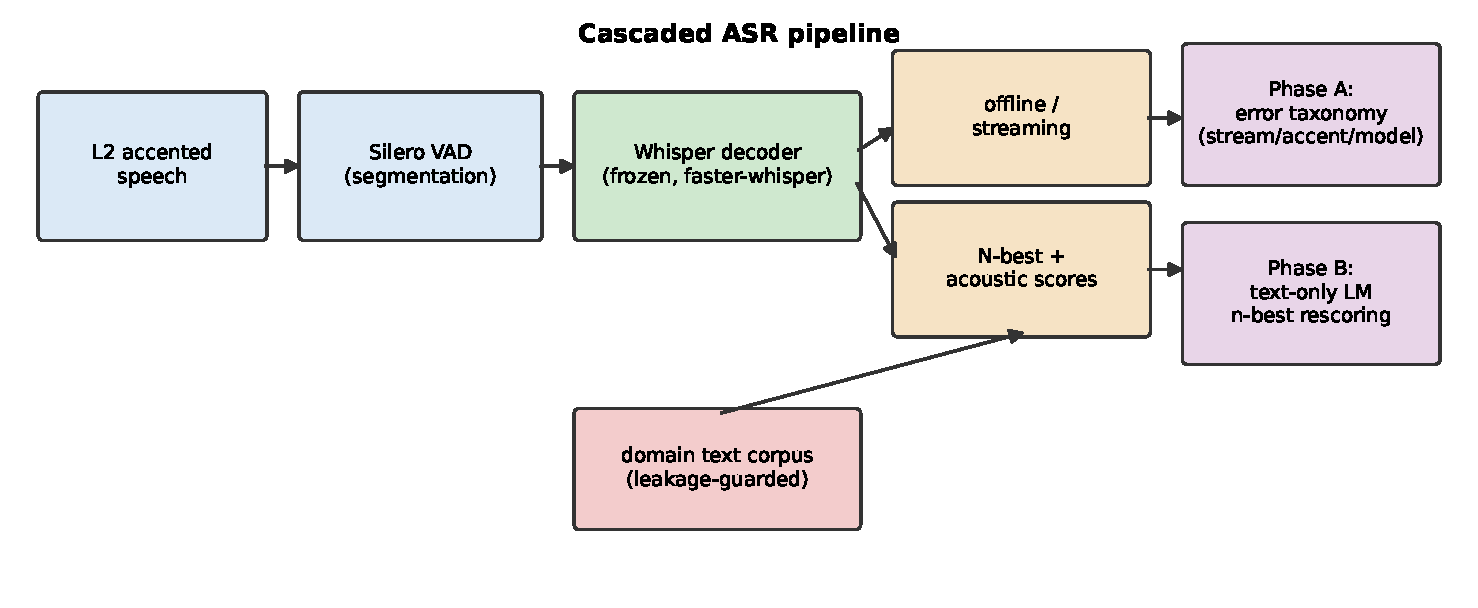
\includegraphics[width=\linewidth]{figures/fig1_pipeline.pdf}
\caption{The cascaded ASR pipeline and the two studies. The Whisper decoder is frozen throughout; Phase~B adds only a text-trained LM at the n-best stage.}
\label{fig:pipeline}
\end{figure}

\subsection{Datasets}
We evaluate on two accented L2 English corpora (Table~\ref{tab:data}). Svarah~\cite{svarah} is Indian-accented English spanning many first languages (L1s) and both read and spontaneous speech. L2-ARCTIC~\cite{l2arctic} is read speech from learners of six L1s with manual phoneme annotations. Under a deliberately resource-constrained setting we evaluate on seeded subsamples. The Phase~B headline adaptation result uses \emph{all 24} L2-ARCTIC speakers (four per L1, 1200 clips); the Phase~A diagnostic and the cross-model-size comparison (Table~\ref{tab:models}) use a fixed six-speaker subset (one per L1), so that the phoneme-aligned error analysis and the model-size differences respectively are not confounded by speaker mix. Audio is resampled to 16~kHz mono.

\begin{table}[t]
\centering
\caption{Evaluation corpora. Subsamples are seeded; clips $<1$\,s (single-word commands) are excluded so streaming chunk effects are well-defined.}
\label{tab:data}
\begin{tabular}{@{}lccc@{}}
\toprule
Property & Svarah & L2-ARCTIC & Role \\
\midrule
Accent / L1s & 19 Indian L1s & 6 L1s & coverage \\
Style & read + spont. & read prompts & domain \\
Phoneme labels & no & yes (manual) & accent truth \\
Phase A clips & 150 & 300 (6 spk) & diagnostic \\
Phase B clips & 150 & 1200 (24 spk, 4/L1) & adaptation \\
\bottomrule
\end{tabular}
\end{table}

\subsection{Phase A: streaming and error diagnostics}
Each clip is decoded under four conditions: offline (full utterance) and streaming with fixed chunks of 1280, 640 and 320~ms. Streaming is emulated by feeding each chunk a bounded left-context window but \emph{no} future audio, isolating the loss of right context; the algorithmic latency equals the chunk size. We report WER and CER (via jiwer~\cite{jiwer}) and real-time factor.

For the error taxonomy, every hypothesis is aligned to its reference and each substitution/deletion/insertion is logged with full reference and hypothesis sentences. Each error is assigned a cause by a transparent, reproducible procedure: (i)~for L2-ARCTIC, errors overlapping an annotated mispronunciation are accent-driven; (ii)~orthographic-only differences (British/American spelling, digit-vs-word numbers, contractions) are normalization; (iii)~when the reference is a substring of the hypothesis (truncated reference), surplus insertions are reference errors; (iv)~repeated insertions are disfluencies and unexplained insertions are hallucinations; remaining substitutions are model-lexical. Accent is asserted \emph{only} from phoneme ground truth. We also tested whether a text-only phonetic-similarity proxy (metaphone identity or Jaro--Winkler $>0.86$) could supply accent labels where phoneme annotations are absent (notably Svarah), but validated against the L2-ARCTIC ground truth the proxy was uncorrelated with the true labels (agreement 49\%, Cohen's $\kappa\approx0$); we therefore do not use it and report no accent share for Svarah. This is an analysis aid, not a substitute for listening (Sec.~\ref{sec:lim}).

\subsection{Phase B: audio-free n-best rescoring}
Phase~B never touches the acoustic model. For each clip we extract the decoder's top-$N$ hypotheses with acoustic scores (via CTranslate2's \texttt{num\_hypotheses}/\texttt{return\_scores}), then re-rank them as
\begin{equation}
\mathrm{score}(h) = s_{\mathrm{ac}}(h) + \lambda \cdot \log P_{\mathrm{LM}}(h)/|h|,
\end{equation}
where the LM term is the per-word log-probability under a domain n-gram model and $\lambda$ is a fusion weight. The LM is a 4-gram trained \emph{only on text}. To prevent leakage---critical because all L2-ARCTIC speakers read the same prompts---every sentence matching a test reference is removed from the LM corpus. $\lambda$ is tuned on a held-out dev split and the WER delta is reported on a disjoint test split, overall and stratified by L1. Choosing $\lambda=0$ recovers the unadapted top-1; but because $\lambda$ is selected on dev, a positive weight can still raise WER on the disjoint test split---precisely what separates the weak from the strong LM below.

\section{Experimental Setup}
The backbone is Whisper-small.en (244\,M parameters) in faster-whisper/CTranslate2, int8 on CPU and float16 on GPU; beam size 5 (offline) and 10 for n-best ($N=10$). We rescore with two LMs of contrasting strength: a weak pure-Python interpolated 4-gram trained on the in-domain corpus, and a strong zero-shot GPT-2 (124\,M) scoring each hypothesis by token log-likelihood. The n-best is decoded once and cached, so both rescorers run cheaply. Phase~A on Svarah ran on an 8\,GB-RAM CPU; the heavier all-condition and n-best decoding ran on a free Colab T4 GPU. Offline WER was identical across CPU (int8) and GPU (float16) decoding (0.132 on Svarah), confirming the hardware swap does not affect results. Scores use jiwer~\cite{jiwer} with light text normalization. For the cross-family generality test (Sec.~\ref{sec:generality}) we additionally decode with wav2vec2-large~\cite{wav2vec2}, obtaining its scored n-best via a CTC beam search; $\lambda$ is tuned on a wider grid there because CTC acoustic scores are scaled differently.

\section{Results}
\subsection{The streaming penalty}
Table~\ref{tab:stream} and Figure~\ref{fig:latwer} show WER rising sharply and monotonically as the chunk shrinks. Relative to offline, 320~ms streaming is $4.8\times$ worse on L2-ARCTIC and $5.3\times$ worse on Svarah. The degradation is driven by the number of chunks, not context length: the encoder pads every chunk to its full window, so smaller chunks impose more recomputation and less right context.

\begin{table}[t]
\centering
\caption{Mean WER/CER by decoding condition. Streaming degrades accuracy monotonically; 320~ms is $\sim5\times$ offline WER on both corpora.}
\label{tab:stream}
\begin{tabular}{@{}lcccc@{}}
\toprule
& \multicolumn{2}{c}{Svarah} & \multicolumn{2}{c}{L2-ARCTIC} \\
\cmidrule(lr){2-3}\cmidrule(lr){4-5}
Condition & WER & CER & WER & CER \\
\midrule
Offline & 0.132 & 0.081 & 0.101 & 0.053 \\
Stream 1280\,ms & 0.364 & 0.211 & 0.199 & 0.121 \\
Stream 640\,ms & 0.477 & 0.291 & 0.304 & 0.196 \\
Stream 320\,ms & 0.705 & 0.451 & 0.480 & 0.310 \\
\bottomrule
\end{tabular}
\end{table}

\begin{figure}[t]
\centering
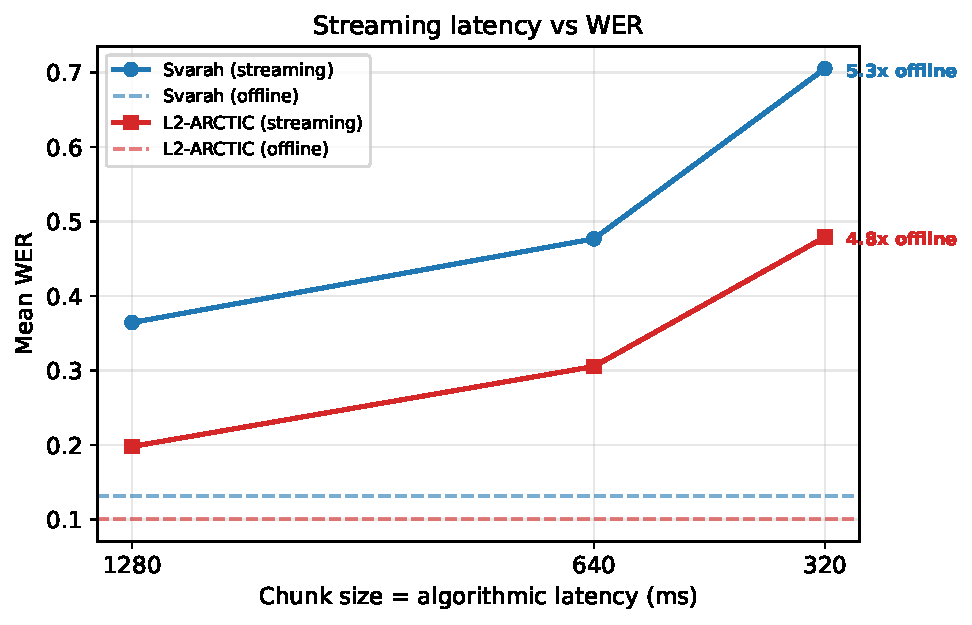
\includegraphics[width=0.92\linewidth]{figures/fig2_latency_wer.pdf}
\caption{Streaming latency vs WER. Dashed lines are offline baselines; markers are streaming conditions (x-axis inverted so latency decreases rightward).}
\label{fig:latwer}
\end{figure}

Figure~\ref{fig:streambreak} shows the failure qualitatively on a real clip: at 320~ms, with no future context, the frozen decoder fragments the sentence and even hallucinates fluent filler, turning a perfect offline transcript into WER~$>1$.

\begin{figure}[t]
\centering
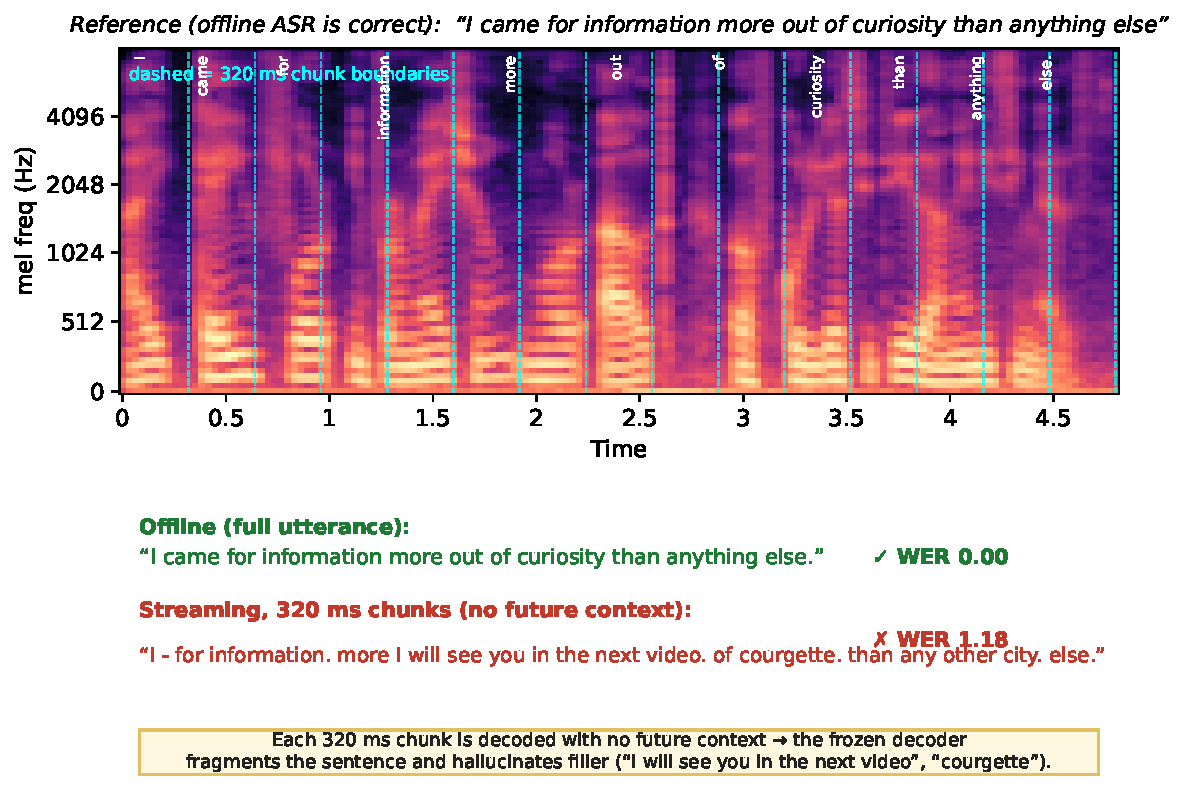
\includegraphics[width=\linewidth]{figures/fig_streaming_break.pdf}
\caption{Streaming breakage on a real L2-ARCTIC clip that offline transcribes perfectly. The mel-spectrogram is overlaid with 320~ms chunk boundaries (dashed) and the offline word alignment; decoded chunk-by-chunk with no future context, the model fragments and hallucinates (``I will see you in the next video'', ``courgette''), WER $0.00 \to 1.18$.}
\label{fig:streambreak}
\end{figure}

\subsection{Accent vs.\ model errors}
Using L2-ARCTIC's phoneme ground truth, 136 of 264 aligned errors (51.5\%) coincide directly with an annotated mispronunciation; the remaining 48.5\% fall on correctly-produced speech. Coincidence varies by operation: 56\% of substitutions and 60\% of deletions are accent-aligned, but only 29\% of insertions---consistent with insertions being hallucinations. The fine taxonomy (Table~\ref{tab:cat}, Figure~\ref{fig:cat}) labels 45.5\% of L2-ARCTIC errors as accent (phoneme-confirmed; some coinciding errors are better explained as normalization or reference errors, which take precedence), the remainder being model-lexical, hallucination, normalization and deletion. \emph{We deliberately report no accent share for Svarah.} Lacking phoneme labels one might substitute a text-only phonetic-similarity proxy (metaphone / Jaro--Winkler), but validated against the L2-ARCTIC ground truth this proxy was uncorrelated with the true accent labels (agreement 49\%, Cohen's $\kappa\approx0$), so we do not use it; Svarah is characterised only by categories text rules determine reliably (model-lexical, hallucination, normalization, deletion).

\begin{table}[t]
\centering
\caption{Error-category composition (offline). L2-ARCTIC accent labels use human phoneme ground truth; Svarah has none, and a text-only phonetic proxy was found uncorrelated with that ground truth (Cohen's $\kappa\approx0$), so no accent share is reported for Svarah (---).}
\label{tab:cat}
\begin{tabular}{@{}lcc@{}}
\toprule
Error category & L2-ARCTIC (\%) & Svarah (\%) \\
\midrule
Accent (phoneme-confirmed) & 45.5 & --- \\
Model lexical & 29.5 & 55.0 \\
Hallucination (insertion) & 11.4 & 21.3 \\
Normalization artifact & 9.1 & 7.5 \\
Deletion (other) & 2.3 & 14.4 \\
Reference error & 2.3 & 1.9 \\
\bottomrule
\end{tabular}
\end{table}

\begin{figure}[t]
\centering
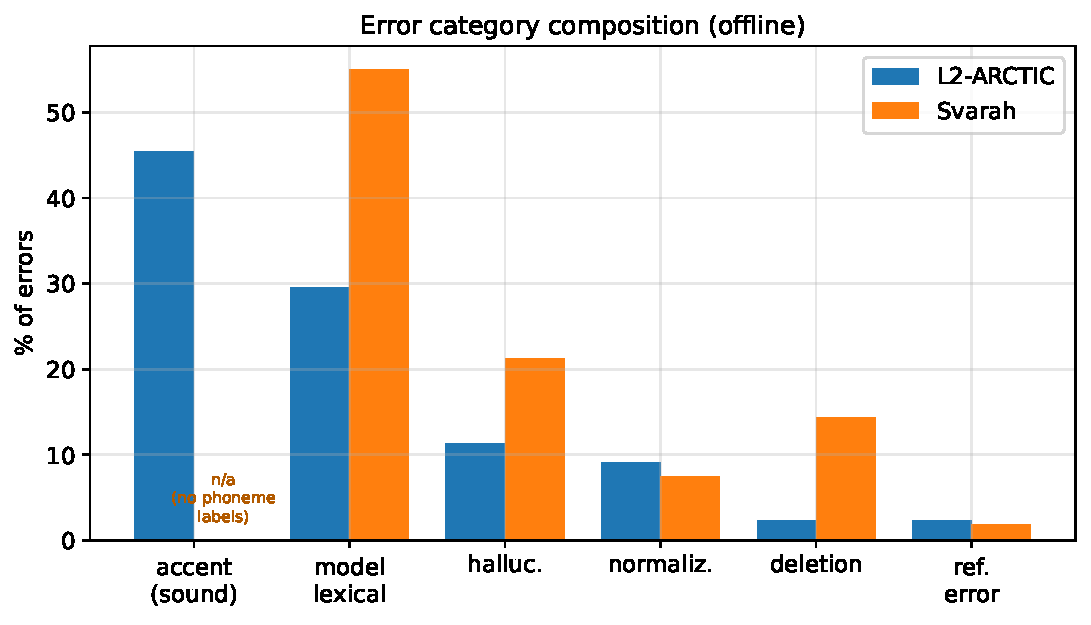
\includegraphics[width=0.95\linewidth]{figures/fig3_error_categories.pdf}
\caption{Error-category composition for both corpora. Only L2-ARCTIC supports a phoneme-confirmed accent category.}
\label{fig:cat}
\end{figure}

\subsection{Audio-free adaptation: it depends on LM strength and speech type}
\label{sec:adapt}
Whether audio-free rescoring helps follows a clean $2\times2$ (Table~\ref{tab:phaseb}, Figure~\ref{fig:phaseb}): the strength of the LM, and whether the speech is read or spontaneous. We rescore the same cached n-best with a weak domain 4-gram and a strong, zero-shot GPT-2.

The weak n-gram never yields a test-set gain. On the six-speaker subset and on Svarah its dev optimum is $\lambda=0$---it cannot out-rank Whisper's internal LM at all---while on the full 24-speaker set the small dev improvement it finds at $\lambda=0.3$ fails to transfer, \emph{raising} test WER by 0.8\% (Figure~\ref{fig:phaseb}, blue star above baseline): a small-corpus n-gram overfits the dev split. The strong neural LM behaves differently. On L2-ARCTIC read speech---evaluated on \emph{all 24 speakers} (four per L1, 1200 clips), which removes the single-speaker-per-L1 confound---its dev gain transfers to test (Figure~\ref{fig:phaseb}, red star below baseline), lowering test WER from 0.084 to 0.077, an 8.0\% relative reduction that improves five of the six L1s. We assess significance with a paired bootstrap. The improvement is significant at the utterance level (tail $p<0.001$) and---crucially---under a \emph{speaker-level} cluster bootstrap that resamples the 24 speakers to account for within-speaker correlation ($p=0.0003$); the speaker-level 95\% CI on the absolute delta, $[-0.011,-0.003]$, excludes zero (two-sided significant at $\alpha=0.05$), so the effect is not an artifact of any single speaker. It is in line with the $\sim$9\% relative gains reported for shallow fusion on attention seq2seq models~\cite{kannan}. The benefit also holds across ASR model size (Table~\ref{tab:models}, Figure~\ref{fig:models}): the GPT-2 gain is significant for tiny.en, base.en and small.en, and is \emph{larger} on the weaker models, which make more lexical errors for the LM to repair. To compare sizes cleanly we hold the speaker set fixed at the six-speaker subset (198 test utterances) for all three models; on this controlled subset small.en gives $-6.4\%$ ($p=0.030$), consistent with---and more conservative than---the $-8.0\%$ it reaches on the full 24 speakers (Table~\ref{tab:phaseb}). A category audit attributes the fixes to lexical error (model-lexical substitutions and number-form normalization), consistent with Table~\ref{tab:examples}. On spontaneous Svarah, even GPT-2 gives no gain ($\Delta=+0.001$, $p=0.74$).

\begin{table}[t]
\centering
\caption{Audio-free n-best rescoring---WER change by LM strength and speech type (test split). Negative = improvement. Adaptation helps in only one cell: a strong LM on read speech.}
\label{tab:phaseb}
\begin{tabular}{@{}lcc@{}}
\toprule
WER $\Delta$ (test) & 4-gram (weak) & GPT-2 (strong) \\
\midrule
L2-ARCTIC (read, 24 spk) & $+0.001$, $+0.8\%$ (n.s.) & $-0.0068$, $-8.0\%$ ($p{<}0.001$) \\
Svarah (spontaneous) & $0.000$ ($\lambda{=}0$) & $+0.0009$, $+0.9\%$ ($p{=}0.74$) \\
\bottomrule
\end{tabular}
\end{table}

\begin{table}[t]
\centering
\caption{Strong-LM (GPT-2) gain across ASR model size, on a \emph{fixed six-speaker} L2-ARCTIC subset (198 test utterances) held constant so that differences reflect model size, not speaker mix. The benefit is significant for every size and larger on the weaker models. On this controlled subset small.en gives $-6.4\%$, versus the $-8.0\%$ headline when small.en is run on all 24 speakers (Table~\ref{tab:phaseb}). ($p$ one-sided bootstrap.)}
\label{tab:models}
\begin{tabular}{@{}lcccc@{}}
\toprule
ASR model & Base WER & Adapt WER & $\Delta$ rel. & $p$ \\
\midrule
tiny.en (39M) & 0.147 & 0.133 & $-9.5\%$ & 0.010 \\
base.en (74M) & 0.124 & 0.109 & $-11.8\%$ & 0.005 \\
small.en (244M) & 0.088 & 0.082 & $-6.4\%$ & 0.030 \\
\bottomrule
\end{tabular}
\end{table}

\begin{figure}[t]
\centering
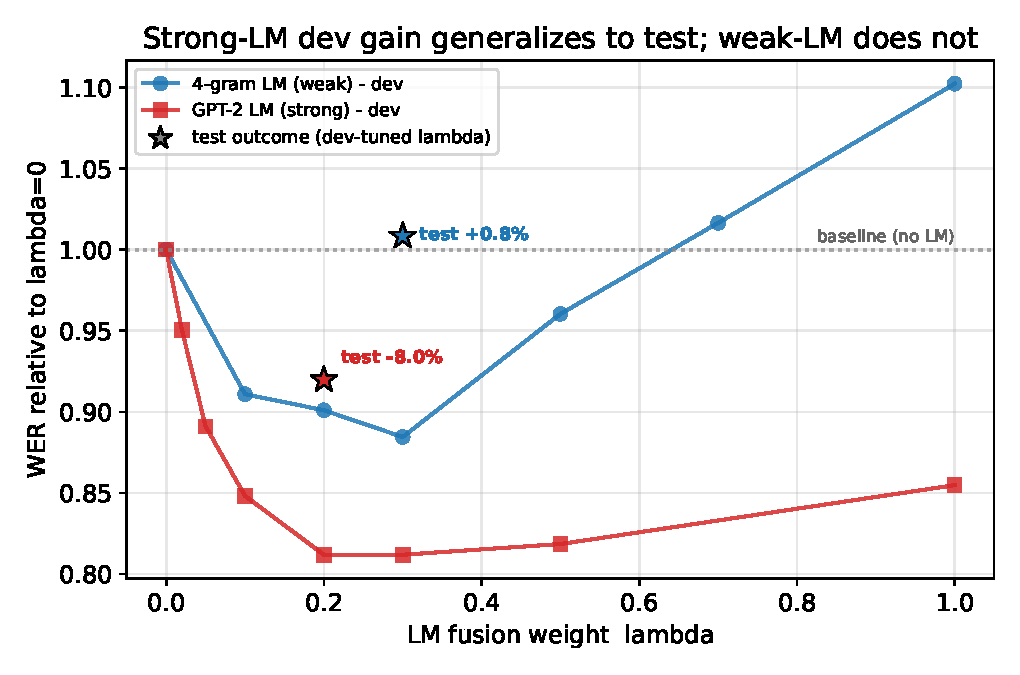
\includegraphics[width=0.92\linewidth]{figures/fig4_phaseB.pdf}
\caption{Dev-set WER versus fusion weight $\lambda$ on L2-ARCTIC (24 speakers); stars mark the realized \emph{test} outcome at each LM's dev-selected $\lambda$. Both LMs lower dev WER, but only the strong GPT-2's gain generalizes (test $-8.0\%$, star below baseline); the weak 4-gram's dev-optimal $\lambda$ \emph{raises} test WER ($+0.8\%$, star above baseline). LM strength decides whether audio-free adaptation transfers.}
\label{fig:phaseb}
\end{figure}

\begin{figure}[t]
\centering
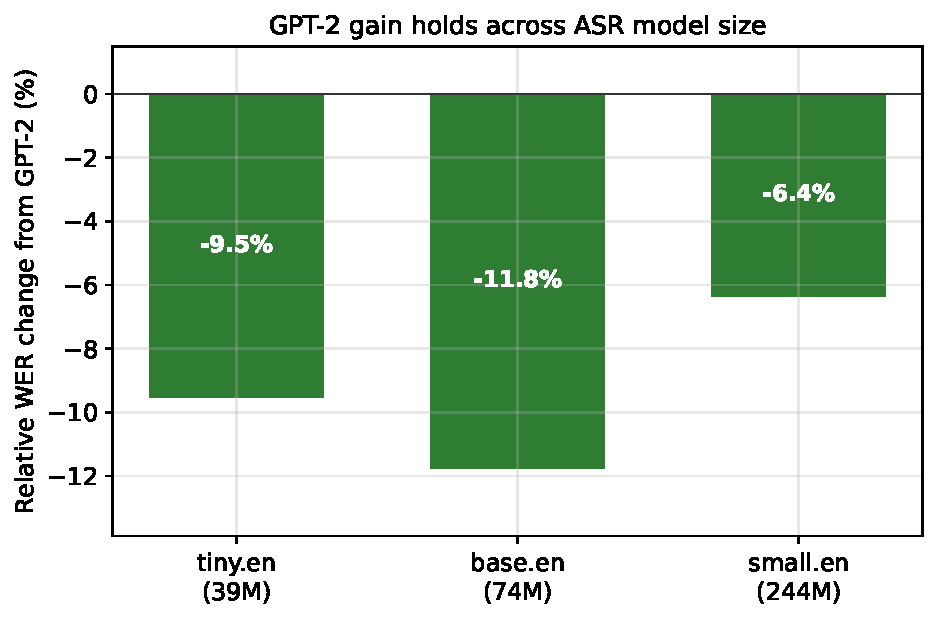
\includegraphics[width=0.86\linewidth]{figures/fig5_model_robustness.pdf}
\caption{Relative WER reduction from GPT-2 rescoring across ASR model size on L2-ARCTIC: significant for all, larger on weaker models.}
\label{fig:models}
\end{figure}

Table~\ref{tab:examples} shows representative GPT-2 corrections: number forms, rare-word recovery, homophone disambiguation from context, and grammatical agreement---the lexical errors a strong LM can identify and the decoder's n-best happens to contain. Figure~\ref{fig:hero} traces one such fix end-to-end: on a real clip the decoder's top acoustic hypothesis mis-hears the homophone ``were'' as ``where'', and the correct wording---ranked only sixth by acoustics---is promoted to first by the LM.

\begin{figure}[t]
\centering
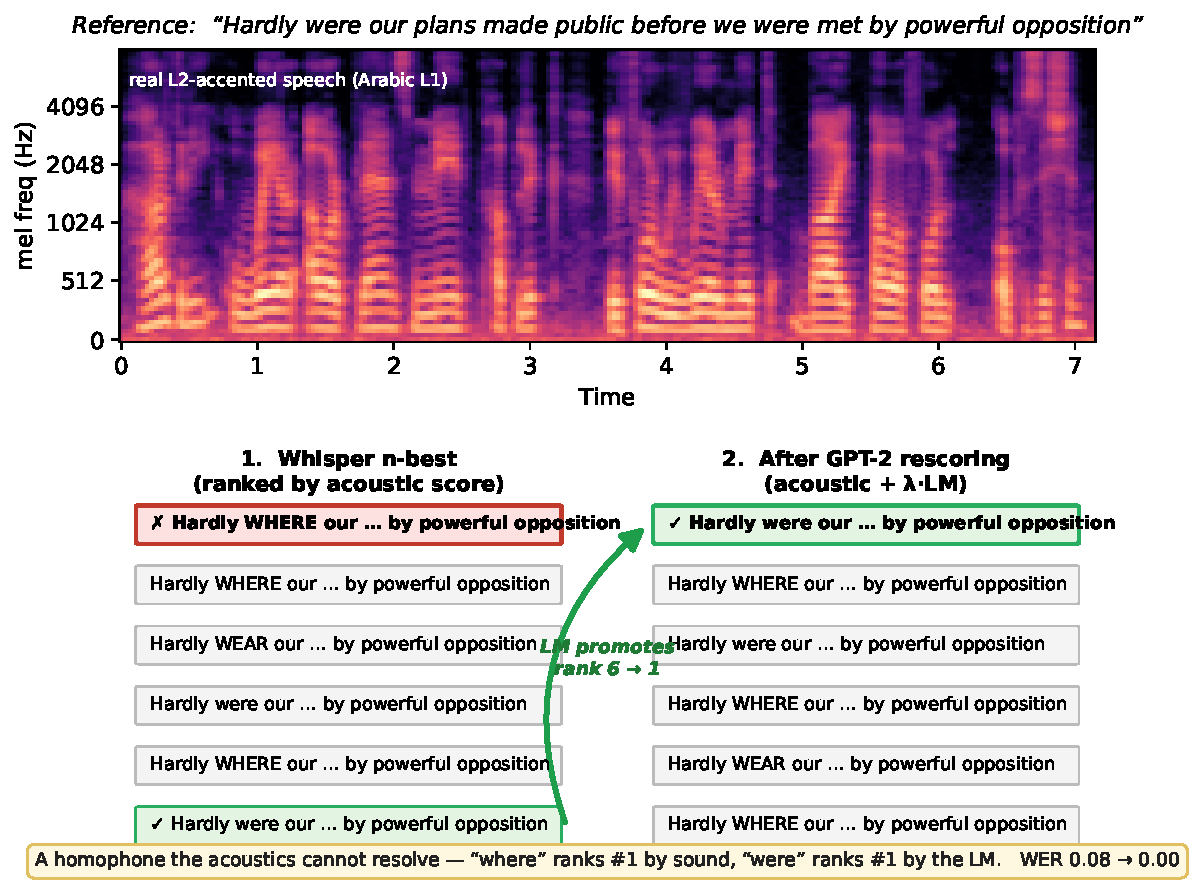
\includegraphics[width=\linewidth]{figures/fig_hero_rescore.pdf}
\caption{How a text LM repairs accented ASR, on a real L2-ARCTIC clip (top: mel-spectrogram). Whisper's acoustic n-best ranks the homophone error ``\textsc{where}'' first; the grammatical wording ``were'' sits sixth by acoustic score but first under acoustic~$+\lambda\cdot$LM, so rescoring promotes it (green arrow). Utterance WER $0.08 \to 0.00$. A sound the acoustics cannot disambiguate, fixed by the language model.}
\label{fig:hero}
\end{figure}

\begin{table}[t]
\centering
\caption{Representative L2-ARCTIC corrections from strong-LM (GPT-2) rescoring.}
\label{tab:examples}
\small
\begin{tabular}{@{}p{0.30\linewidth}p{0.30\linewidth}p{0.30\linewidth}@{}}
\toprule
Reference & Baseline & Adapted \\
\midrule
three hundred yards & 300 yards & three hundred yards \\
the handkerchief & the hand crochet & the handkerchief \\
the fourth and fifth & the 4th and 5th & the fourth and fifth \\
the gray eyes & the gray ice & the gray eyes \\
there would have & there will have & there would have \\
\bottomrule
\end{tabular}
\end{table}

\subsection{How much error is recoverable? An oracle ceiling and an LM-strength ladder}
\label{sec:ceiling}
How much of the residual error can \emph{any} audio-free rescorer reach? We answer with two analyses on the same 24-speaker test split, both purely on the cached n-best (no audio).

\textbf{Oracle ceiling.} If an oracle always picked the lowest-WER hypothesis in the top-10, test WER would fall from 0.084 to 0.042---\emph{half} the error is already present, correctly transcribed, somewhere in the n-best (Figure~\ref{fig:oracle}). The recoverable fraction grows monotonically with depth (WER $0.073/0.062/0.053/0.042$ at $N=2/3/5/10$) and has not saturated at ten. The bottleneck is therefore not that the decoder lacks the right words, but that selecting them needs information the top-1 acoustic ranking lacks.

\textbf{LM-strength ladder.} Does a stronger LM climb toward this ceiling? We rescore the identical n-best with a ladder of LMs from a 4-gram to GPT-2-xl, taking each LM's word-level perplexity on the held-out references as its strength (Table~\ref{tab:ladder}, Figure~\ref{fig:ladder}). The gain rises smoothly as the LM strengthens---$+0.8\%$ (the 4-gram \emph{hurts}), $-3.3\%$, $-8.0\%$, $-11.9\%$---and then \emph{saturates}: GPT-2-medium (355\,M), large (774\,M) and xl (1.5\,B) are essentially tied at $\approx-12\%$, so a $4\times$ increase in LM size past medium buys nothing. The plateau captures only $\approx24\%$ of the oracle-recoverable head-room; the other $\approx76\%$ sits in the n-best but is invisible to text, because the cue that distinguishes the correct hypothesis is acoustic, not lexical. This is the quantitative form of the accent bound: the ceiling on audio-free adaptation is set by acoustics, not by LM capacity. (The significance-tested $-8.0\%$ of Sec.~\ref{sec:adapt} corresponds to the GPT-2-124M rung; the larger LMs only deepen the effect.)

\textbf{Fine-tuning vs.\ scale.} A GPT-2 (124\,M) fine-tuned on the leakage-guarded in-domain corpus---whose training text shares no sentence with any test prompt---reaches $-11.4\%$, matching GPT-2-medium, a model $3\times$ larger, and the plateau (Table~\ref{tab:ladder}). Genuine, audio-free domain adaptation thus delivers what scale does at a fraction of the cost, but neither breaks the acoustic ceiling.

\begin{table}[t]
\centering
\caption{LM-strength ladder on L2-ARCTIC (24 speakers, test split). Strength = word-level perplexity on held-out references (lower is stronger). The gain scales with strength then saturates by GPT-2-medium; a fine-tuned 124\,M model matches a $3\times$-larger general model. Head-room~\% is the fraction of the oracle-recoverable error (baseline$\to$0.042) captured.}
\label{tab:ladder}
\small
\begin{tabular}{@{}lrcrr@{}}
\toprule
LM & ppl & $\lambda^\ast$ & $\Delta$ rel. & head-room \\
\midrule
4-gram (weak)            & 1017 & 0.3 & $+0.8\%$  & $-2\%$ \\
distilGPT-2 (82\,M)       & 134  & 0.2 & $-3.3\%$  & $7\%$ \\
GPT-2 (124\,M)            & 67   & 0.2 & $-8.0\%$  & $16\%$ \\
GPT-2-medium (355\,M)     & 54   & 0.3 & $-11.9\%$ & $24\%$ \\
GPT-2-large (774\,M)      & 49   & 0.2 & $-11.9\%$ & $24\%$ \\
GPT-2-xl (1.5\,B)         & 47   & 0.2 & $-11.5\%$ & $23\%$ \\
GPT-2 fine-tuned (124\,M) & 54   & 0.3 & $-11.4\%$ & $23\%$ \\
\bottomrule
\end{tabular}
\end{table}

\begin{figure}[t]
\centering
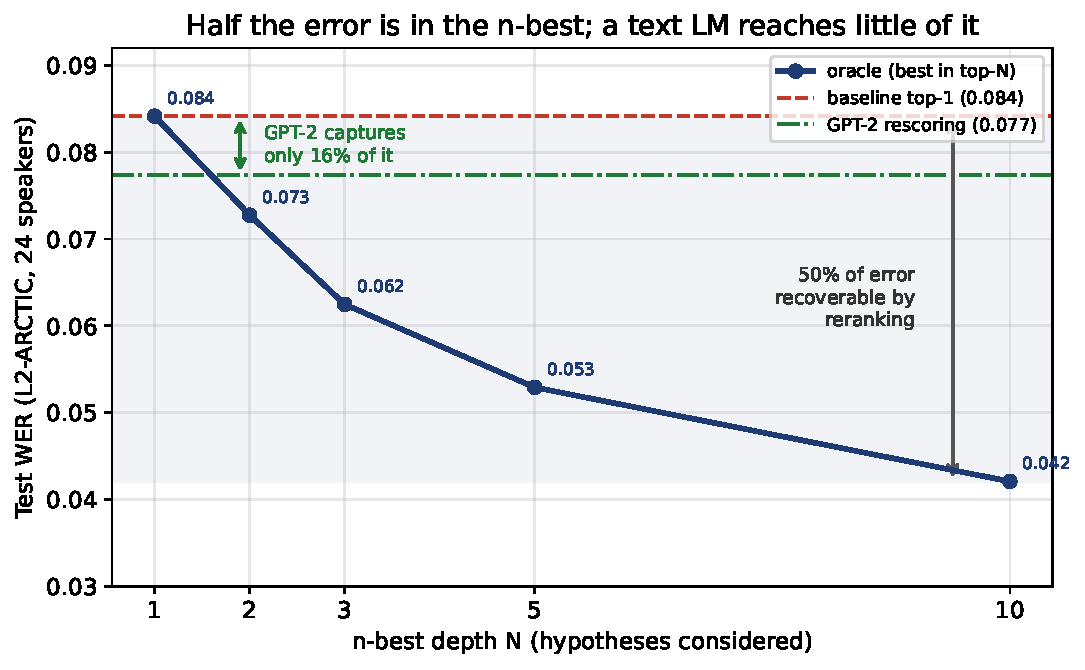
\includegraphics[width=\linewidth]{figures/fig_oracle_headroom.pdf}
\caption{Half the error is recoverable from the n-best: an oracle picking the best of the top-$N$ hypotheses reaches WER 0.042 (from 0.084), and recoverability keeps growing with depth. A strong text LM (GPT-2) captures only $\approx16\%$ of this head-room---the rest is acoustic/accent error that sits in the list but is invisible to a language model.}
\label{fig:oracle}
\end{figure}

\begin{figure}[t]
\centering
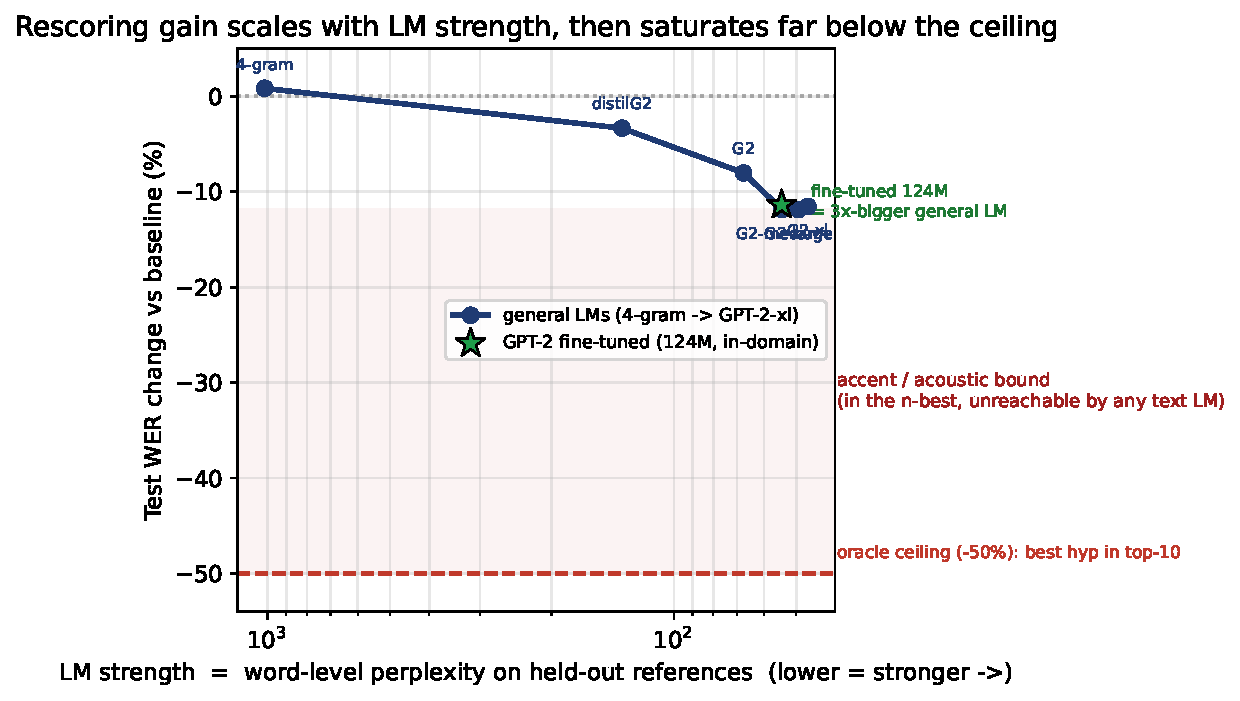
\includegraphics[width=\linewidth]{figures/fig_lm_ladder.pdf}
\caption{Rescoring gain versus LM strength (word-level perplexity, stronger rightward). The gain scales with LM strength then saturates at $\approx-12\%$, far above the $-50\%$ oracle ceiling; the shaded band is the accent/acoustic error that no text LM reaches. A fine-tuned 124\,M model (star) reaches the same plateau as a 1.5\,B general model.}
\label{fig:ladder}
\end{figure}

\subsection{Why it helps read speech but not spontaneous speech}
The two phases explain the $2\times2$. A text-only LM can only adjudicate between hypotheses that differ in their words, and only if a better wording is in the n-best. Two things must align. First, the LM must be strong enough to score natural English: the small-corpus 4-gram cannot beat Whisper's internal LM and only adds noise, whereas GPT-2 carries enough knowledge to prefer the correct wording. Second, the errors must be lexical and a better hypothesis must be present: on L2-ARCTIC read speech enough errors are lexical (number forms, rare words, contextual homophones) for a strong LM to help; on spontaneous Svarah, errors are more acoustic and varied and the n-best rarely contains a better wording, so even GPT-2 cannot help. The gain is real and robust where it occurs but inherently bounded: about half of errors are accent-driven (51\% by phoneme ground truth) and beyond any text model, which is why even the strong-LM benefit caps in the single-digit-to-low-teens percent range and disappears on spontaneous speech. Audio-free adaptation is thus a cheap, effective complement for strong-LM read-speech settings, not a general substitute for acoustic-side adaptation.

\subsection{Generality across ASR families: wav2vec2}
\label{sec:generality}
Are these findings specific to Whisper? We repeat Phase B on a second, architecturally distinct family---wav2vec2-large, a self-supervised \emph{CTC} model---decoding its scored n-best with a CTC beam search and applying the identical rescoring, oracle and significance pipeline (Table~\ref{tab:family}). The strong-LM read-speech gain reproduces only \emph{directionally} ($-3.0\%$), and the cross-family comparison is more revealing than a clean replication: two properties, both read off our own framework, explain the divergence. First, the \textbf{recoverable head-room differs}---wav2vec2's CTC n-best is far less lexically diverse, with an oracle ceiling of only 26\% versus Whisper's 50\%, so there is little for any LM to exploit, bounding the gain. Second, wav2vec2 (CTC) has \textbf{no internal LM}, so even the weak 4-gram helps it ($-4.6\%$), whereas the same n-gram \emph{hurts} Whisper, whose attention decoder already carries a strong internal LM. Consequently \emph{LM strength barely matters} on wav2vec2---the weak n-gram ($-4.6\%$) and GPT-2 ($-3.0\%$) are comparable and neither is speaker-level significant (GPT-2 $p=0.12$)---in sharp contrast to Whisper, where LM strength is decisive and the GPT-2 gain is robust ($-8.0\%$, $p=0.0003$). Audio-free rescoring is therefore \emph{architecture-dependent} in a way the oracle bound and the internal-LM distinction together predict: the recoverable head-room bounds how much any LM can gain, while the presence of an internal LM determines whether a strong LM is required or a weak one suffices. The single-system claim ``a strong LM helps'' is thus incomplete; the cross-family view turns it into a predictive account of \emph{when} and \emph{what kind of} text-only adaptation helps.

\begin{table}[t]
\centering
\caption{Phase B across two ASR families (L2-ARCTIC, 24 speakers, test split). The oracle head-room bounds the gain's magnitude; the internal LM determines whether a weak LM suffices. $\Delta$ is relative WER at the dev-tuned $\lambda$.}
\label{tab:family}
\begin{tabular}{@{}lcccc@{}}
\toprule
ASR family & Base WER & oracle & 4-gram $\Delta$ & GPT-2 $\Delta$ \\
\midrule
Whisper-small (attn.\ enc--dec) & 0.084 & 50\% & $+0.8\%$ (n.s.) & $-8.0\%$ ($p{<}0.001$) \\
wav2vec2-large (CTC) & 0.070 & 26\% & $-4.6\%$ & $-3.0\%$ (n.s.) \\
\bottomrule
\end{tabular}
\end{table}

\section{Discussion}
Three implications follow. First, for streaming deployment on accented speech, chunk size is a first-order accuracy lever: moving from 1280~ms to 320~ms roughly doubles WER, so latency budgets should be set with accented users in mind. Second, headline WER conflates failure modes; the $\sim$50/50 accent-vs-model split means nearly half of ``accent errors'' are model errors that better acoustic modelling---not pronunciation training---would fix. Third, audio-free text adaptation is a useful, cheap complement \emph{when used correctly}: a strong neural LM gives a significant read-speech WER reduction that holds across 24 speakers and across ASR model sizes, but it requires a strong LM (a domain n-gram is useless), helps only where errors are lexical (read, not spontaneous speech), and is bounded by the accent/acoustic errors that dominate. It complements rather than replaces acoustic-side adaptation. Methodologically, our evaluation is a caution in both directions: one speaker per language can mislead either way---a partial three-L1 subset earlier produced a spurious 15.5\% gain that vanished, while the six-speaker test understated an effect that strengthened and reached high significance only on 24 speakers---so full speaker/L1 coverage and speaker-level significance testing are essential.

\section{Limitations}
\label{sec:lim}
\begin{itemize}
\item Scale: results use seeded subsamples; the read-speech effect is now confirmed on all 24 L2-ARCTIC speakers (four per L1, speaker-level $p=0.0003$) and across three ASR model sizes, but the corpora remain modest in size and English-only, and Svarah is evaluated on 150 clips. The cross-family generality test (wav2vec2) is on one read corpus, and its single-LM gain---though directionally consistent and mechanistically explained---is not robustly significant; broader replication across families and corpora would further tighten the account. Larger and more diverse evaluation would further tighten the estimates.
\item Annotation: error categorization is semi-automated. L2-ARCTIC accent labels rest on human phoneme annotations; we tested a text-only phonetic proxy for use where such labels are absent (Svarah) but found it uncorrelated with the ground truth (Cohen's $\kappa\approx0$), so we report no accent share for Svarah. The remaining labels are conservative text rules. An automated faithfulness audit finds 94.3\% of the 264 labels satisfy their definitional rule, and a manual re-adjudication of a stratified 50-error sample agreed with the automatic labels in 88\% (44/50) of cases. The disagreements concentrate at two boundaries the text rules handle crudely: number-format strings (``three hundred''/``300'') tagged as deletion or accent rather than normalization, and word-splitting insertions (e.g.\ ``Anyway''$\to$``in a way'') tagged as hallucination---neither of which affects the accent-vs-model headline, which rests on the phoneme ground truth. We release the full 50-error sheet (with audio and seek times) for independent validation; labels are text-level, not audio-perceptually verified.
\item LMs tested span a domain 4-gram, zero-shot GPT-2 from 82\,M to 1.5\,B, and a fine-tuned in-domain GPT-2; all \emph{re-rank} the fixed n-best. We did not test first-pass shallow fusion, nor \emph{generative} error correction, in which an LLM rewrites the transcript and can recover words absent from the n-best, surpassing the re-ranking oracle~\cite{hyporadise,whisperingllama,gensec}. That route may break the acoustic ceiling we report, at substantially higher cost; whether it also overcomes the spontaneous-speech null is an open question.
\end{itemize}

\section{Conclusion}
We presented a diagnostic-then-adaptation study of cascaded ASR on accented learner speech. Streaming imposes a large, monotonic penalty (up to $\sim5\times$ WER); about half of L2-ARCTIC errors are genuine accent mispronunciations and half are model errors on correctly-produced speech; and audio-free n-best rescoring helps only when two conditions hold---a strong LM and lexically-fixable read speech. A weak n-gram yields no test gain (its dev improvement does not transfer); a strong GPT-2 cuts L2-ARCTIC read-speech WER by 8.0\% relative across 24 speakers (speaker-level $p=0.0003$), a gain that holds across ASR model sizes, but does nothing for spontaneous Svarah. The error taxonomy explains the pattern: text fixes lexical errors but not the acoustic, accent-driven errors that dominate. Audio-free adaptation is thus a cheap, effective complement in the right setting---not a general substitute for acoustic-side methods. We release the full pipeline---diagnostics, taxonomy, rescoring, and significance testing---to support reproducible, honestly-evaluated work on equitable ASR for second-language speakers.

\section{Ethics Statement}
This work uses only publicly released, consented speech corpora (Svarah and L2-ARCTIC) under their respective research licenses; no new human-subjects data were collected. The study is motivated by equity: ASR systematically underserves accented and second-language speakers~\cite{koenecke,tatman}, and our diagnostics are intended to help close that gap rather than to profile speakers. We report a negative-leaning result honestly (a weak LM yields no usable gain; a strong LM helps only read speech, modestly) to avoid overstating cheap fixes. No audio is redistributed; only derived metrics and code are released. Speaker first-language labels are used solely for aggregate fairness analysis.

\section{Reproducibility and Data Availability}
All code, configuration, and derived results (WER/CER tables, error taxonomies, rescoring outputs, significance estimates) are released under an MIT license and archived on Zenodo (DOI:~\texttt{10.5281/zenodo.20817700}). No audio is included: each dataset is fetched from its official source by a provided script and converted to a common format. Random subsampling, dev/test splits, and bootstrap resampling use fixed seeds. The Phase~A streaming sweep runs on an 8\,GB-RAM CPU; the all-condition and n-best decoding run on a single free-tier T4 GPU. Offline WER matched across CPU (int8) and GPU (float16) decoding, confirming hardware-independence of the reported numbers.

\section*{Acknowledgments}
We thank the AI4Bharat and Texas A\&M PSI teams for releasing the Svarah and L2-ARCTIC corpora, and the maintainers of faster-whisper, CTranslate2, and Hugging Face Transformers.

\begin{thebibliography}{99}
\bibitem{whisper} A.~Radford \emph{et al.}, ``Robust Speech Recognition via Large-Scale Weak Supervision,'' in \emph{Proc. ICML}, 2023.
\bibitem{svarah} T.~Javed \emph{et al.}, ``Svarah: Evaluating English ASR Systems on Indian Accents,'' in \emph{Proc. Interspeech}, 2023.
\bibitem{l2arctic} G.~Zhao, S.~Sonsaat, A.~Silpachai, I.~Lucic, E.~Chukharev-Hudilainen, J.~Levis, and R.~Gutierrez-Osuna, ``L2-ARCTIC: A Non-native English Speech Corpus,'' in \emph{Proc. Interspeech}, 2018.
\bibitem{arctic} J.~Kominek and A.~W. Black, ``The CMU ARCTIC Speech Databases,'' in \emph{Proc. ISCA Speech Synthesis Workshop}, 2004.
\bibitem{koenecke} A.~Koenecke, A.~Nam, E.~Lake, J.~Nudell, M.~Quartey, Z.~Mengesha, C.~Toups, J.~R. Rickford, D.~Jurafsky, and S.~Goel, ``Racial Disparities in Automated Speech Recognition,'' \emph{Proc. National Academy of Sciences}, vol.~117, no.~14, pp.~7684--7689, 2020.
\bibitem{tatman} R.~Tatman, ``Gender and Dialect Bias in YouTube's Automatic Captions,'' in \emph{Proc. Workshop on Ethics in NLP}, 2017.
\bibitem{ctc} A.~Graves, S.~Fern\'andez, F.~Gomez, and J.~Schmidhuber, ``Connectionist Temporal Classification: Labelling Unsegmented Sequence Data with Recurrent Neural Networks,'' in \emph{Proc. ICML}, 2006.
\bibitem{las} W.~Chan, N.~Jaitly, Q.~Le, and O.~Vinyals, ``Listen, Attend and Spell,'' in \emph{Proc. ICASSP}, 2016.
\bibitem{conformer} A.~Gulati \emph{et al.}, ``Conformer: Convolution-augmented Transformer for Speech Recognition,'' in \emph{Proc. Interspeech}, 2020.
\bibitem{he2019} Y.~He \emph{et al.}, ``Streaming End-to-End Speech Recognition for Mobile Devices,'' in \emph{Proc. ICASSP}, 2019.
\bibitem{wav2vec2} A.~Baevski, H.~Zhou, A.~Mohamed, and M.~Auli, ``wav2vec 2.0: A Framework for Self-Supervised Learning of Speech Representations,'' in \emph{Proc. NeurIPS}, 2020.
\bibitem{hubert} W.-N. Hsu, B.~Bolte, Y.-H.~H. Tsai, K.~Lakhotia, R.~Salakhutdinov, and A.~Mohamed, ``HuBERT: Self-Supervised Speech Representation Learning by Masked Prediction of Hidden Units,'' \emph{IEEE/ACM Trans. Audio, Speech, Lang. Process.}, vol.~29, 2021.
\bibitem{wittyoung} S.~M. Witt and S.~J. Young, ``Phone-Level Pronunciation Scoring and Assessment for Interactive Language Learning,'' \emph{Speech Communication}, vol.~30, no.~2--3, pp.~95--108, 2000.
\bibitem{mdd} W.-K. Leung, X.~Liu, and H.~Meng, ``CNN-RNN-CTC Based End-to-End Mispronunciation Detection and Diagnosis,'' in \emph{Proc. ICASSP}, 2019.
\bibitem{fusion} C.~Gulcehre \emph{et al.}, ``On Using Monolingual Corpora in Neural Machine Translation,'' \emph{arXiv:1503.03535}, 2015.
\bibitem{kannan} A.~Kannan, Y.~Wu, P.~Nguyen, T.~N. Sainath, Z.~Chen, and R.~Prabhavalkar, ``An Analysis of Incorporating an External Language Model into a Sequence-to-Sequence Model,'' in \emph{Proc. ICASSP}, 2018.
\bibitem{kenlm} K.~Heafield, ``KenLM: Faster and Smaller Language Model Queries,'' in \emph{Proc. WMT}, 2011.
\bibitem{gpt2} A.~Radford, J.~Wu, R.~Child, D.~Luan, D.~Amodei, and I.~Sutskever, ``Language Models are Unsupervised Multitask Learners,'' OpenAI Technical Report, 2019.
\bibitem{transformer} A.~Vaswani \emph{et al.}, ``Attention Is All You Need,'' in \emph{Proc. NeurIPS}, 2017.
\bibitem{bisani} M.~Bisani and H.~Ney, ``Bootstrap Estimates for Confidence Intervals in ASR Performance Evaluation,'' in \emph{Proc. ICASSP}, 2004.
\bibitem{koehn} P.~Koehn, ``Statistical Significance Tests for Machine Translation Evaluation,'' in \emph{Proc. EMNLP}, 2004.
\bibitem{silero} Silero Team, ``Silero VAD: Pre-trained Enterprise-Grade Voice Activity Detector,'' GitHub, 2021.
\bibitem{fasterwhisper} SYSTRAN, ``faster-whisper: Fast Inference for Whisper Using CTranslate2,'' GitHub, 2023.
\bibitem{jiwer} N.~Vaessen \emph{et al.}, ``jiwer: Evaluate ASR with WER/CER,'' software, 2018.
\bibitem{hyporadise} C.~Chen, Y.~Hu, C.-H.~H. Yang, S.~M. Siniscalchi, P.-Y. Chen, and E.~S. Chng, ``HyPoradise: An Open Baseline for Generative Speech Recognition with Large Language Models,'' in \emph{Proc. NeurIPS Datasets and Benchmarks Track}, 2023.
\bibitem{whisperingllama} S.~Radhakrishnan, C.-H.~H. Yang, S.~A. Khan, R.~Kumar, N.~A. Kiani, D.~Gomez-Cabrero, and J.~N. Tegner, ``Whispering LLaMA: A Cross-Modal Generative Error Correction Framework for Speech Recognition,'' in \emph{Proc. EMNLP}, 2023.
\bibitem{gensec} C.-H.~H. Yang \emph{et al.}, ``Large Language Model Based Generative Error Correction: A Challenge and Baselines for Speech Recognition, Speaker Tagging, and Emotion Recognition,'' \emph{arXiv:2409.09785}, 2024.
\end{thebibliography}

\end{document}
